Кодировщик выдает нам $\mu$ и $\sigma$ и мы по ним генерируем какой-то вектор $z$ из этого распределения. Проблема: непонятно, как посчитать производную производную выхода по $\mu$ и $\sigma$, поскольку там происходит вероятностный процесс. Вместо этого сделаем так:

Кодировщик выдает нам $\mu$ и $\sigma$ (это конкретные детерминированные числа), а еще мы будем генерировать стандартное нормальное число $\varepsilon$. И чтобы получить конкретное представление $z$ мы сделаем $z = \mu + \sigma \odot \varepsilon$ (здесь $\odot$ --- поэлементное умножение). То есть фактически мы разделяем случайность (запихиваем ее в $\varepsilon$), при этом делая ее без параметров (и никакие градиенты туда не нужны), и выдачу параметров кодировщиком (см. рисунок \ref{fig:5_reparameterization} в качестве иллюстрации).

\begin{figure}[H]
	\centering
	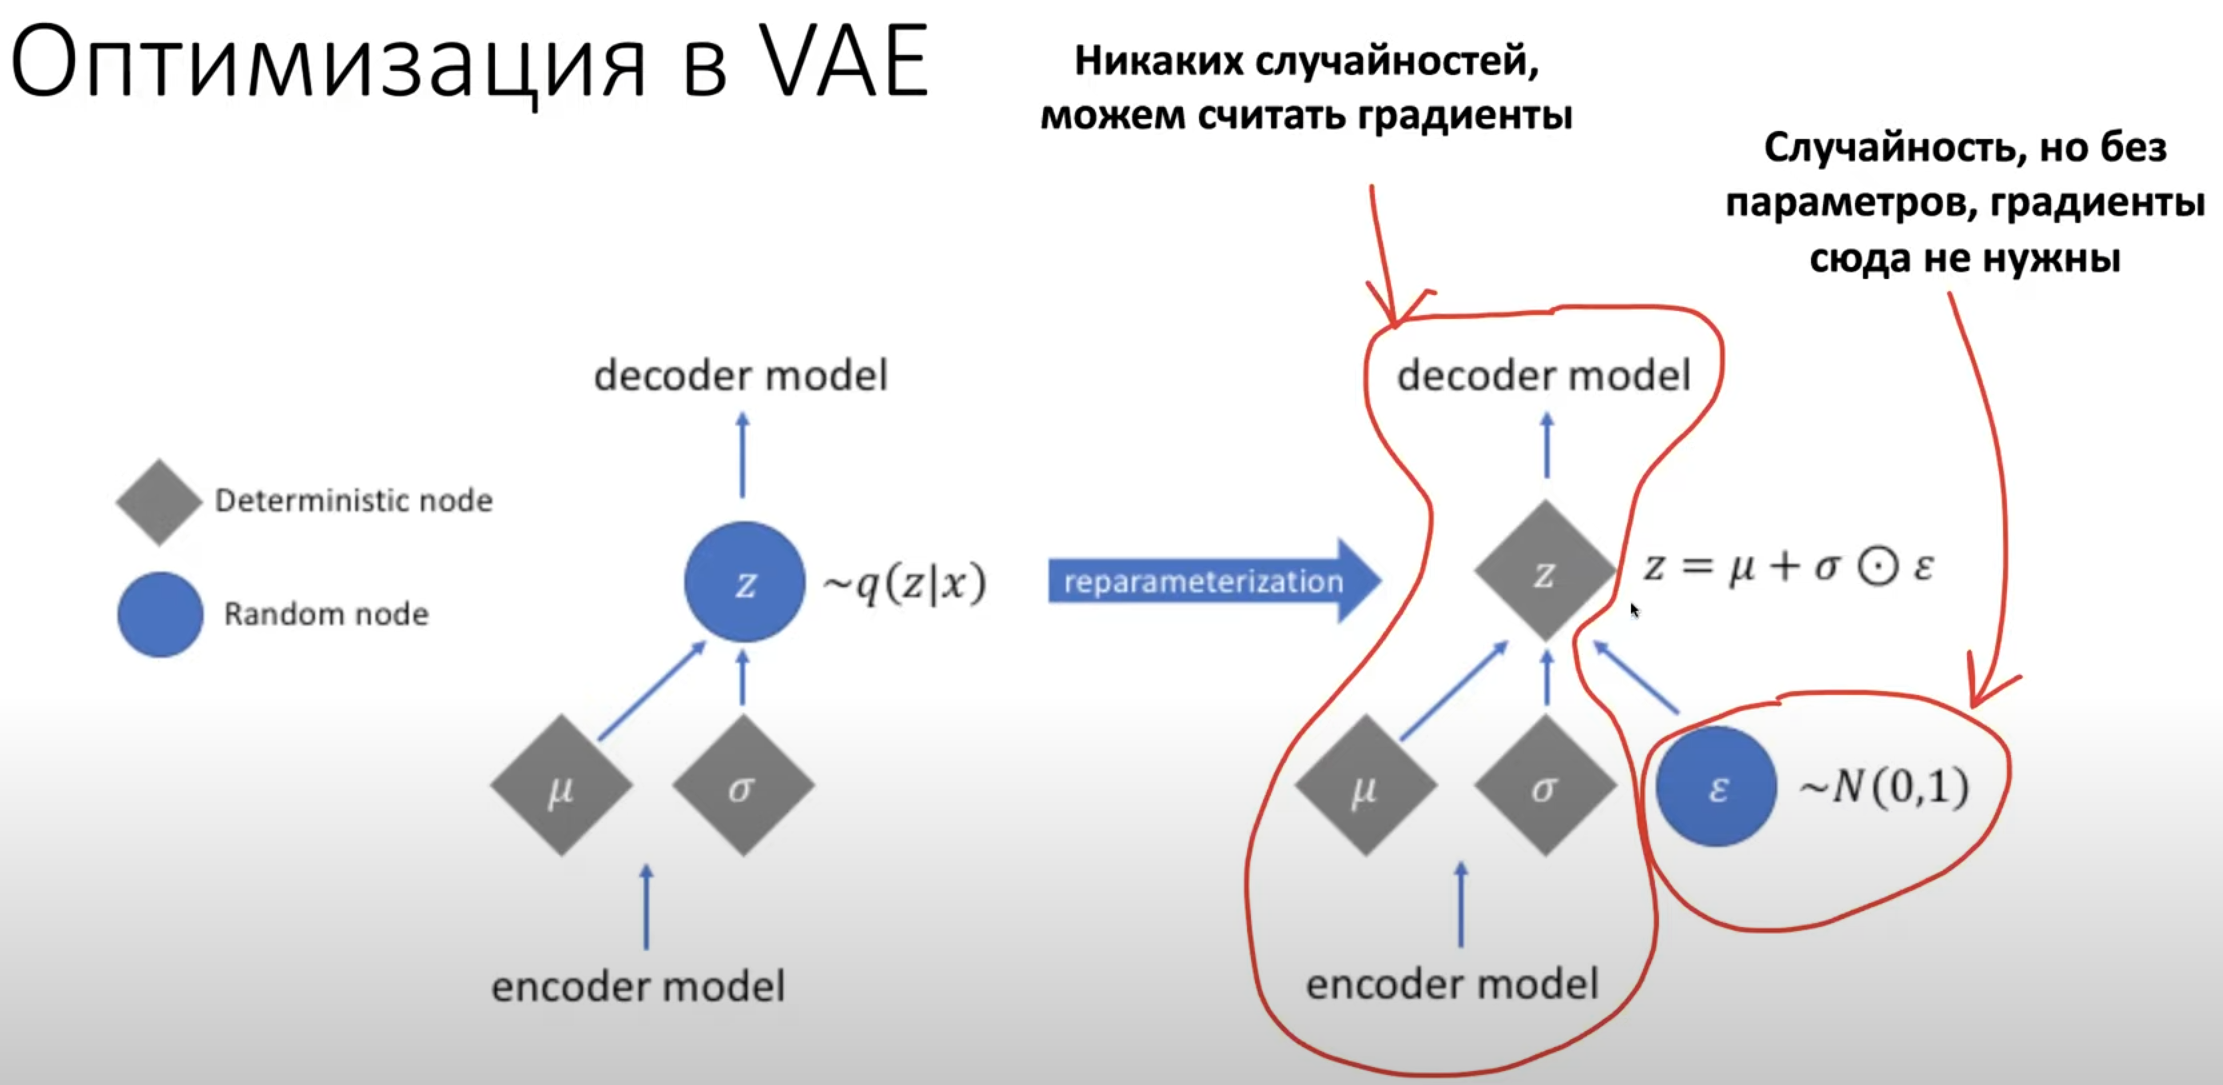
\includegraphics[width=\linewidth]{5_reparameterization}
	\caption{Трюк репараметризации (слева без него, справа с ним)}
	\label{fig:5_reparameterization}
\end{figure}